Domain is periodic and a hydrostatic force is acting in the direction of the arrows:
positive in one half of the domain and negative in the other half.  Red
particles are $100$ times for viscous. Particles are immiscible on the
right and fully miscible on the left. Arrows are velocity fields: red
particles have almost flat velocity profile.
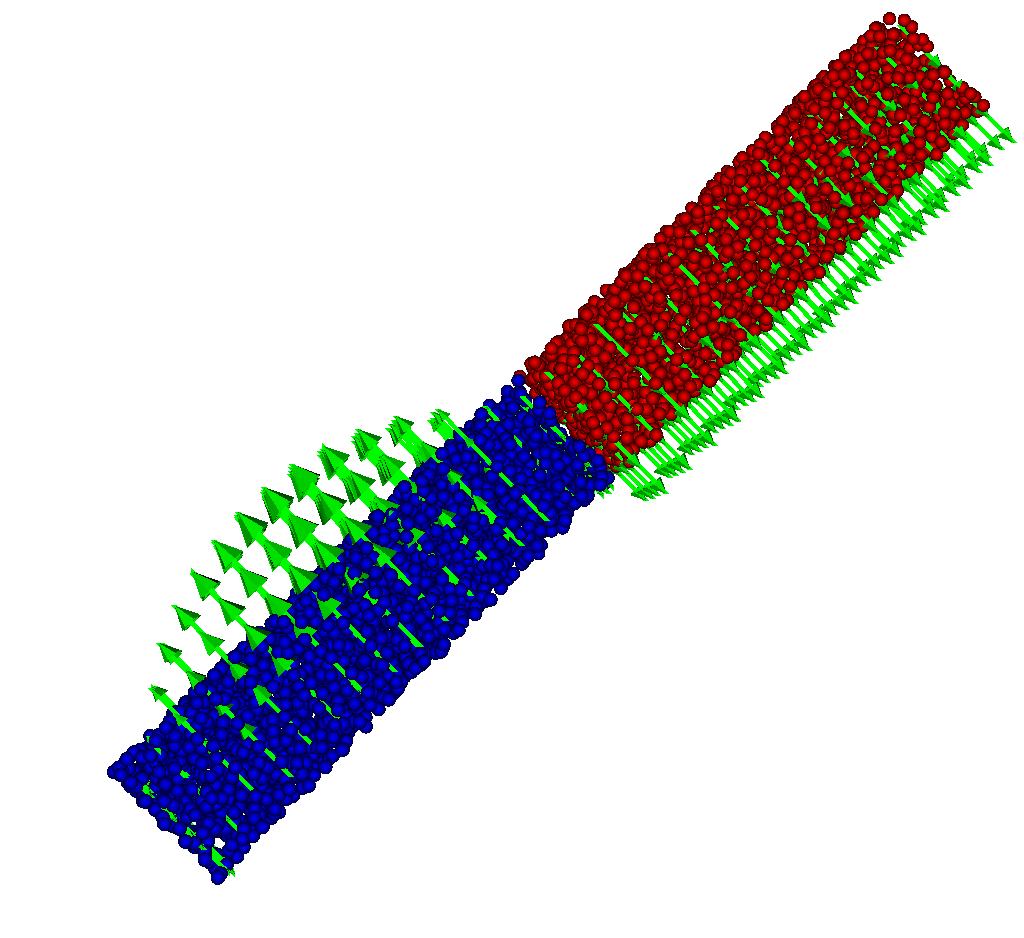
\includegraphics[width=0.5\textwidth]{i/flow/a/visit.png}
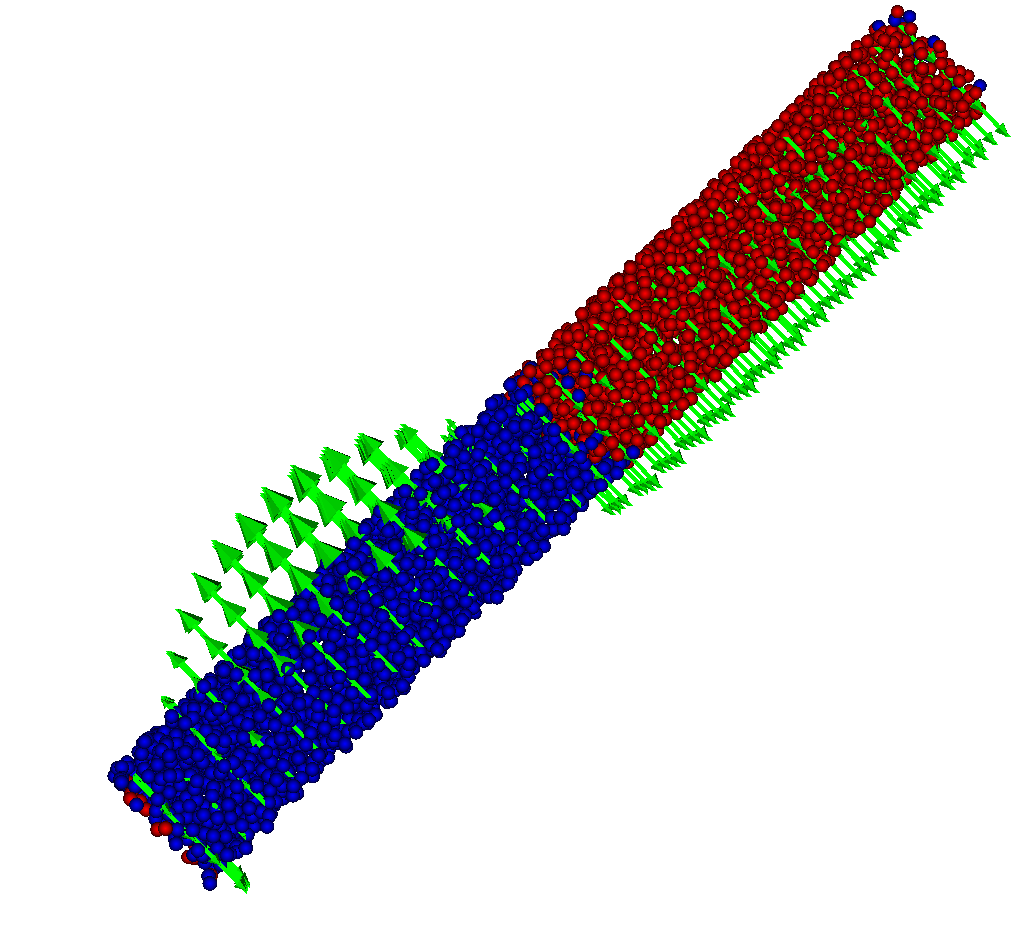
\includegraphics[width=0.5\textwidth]{i/flow/b/visit.png}


The average velocity fields are shown below. ``Immicible'' case is
more ``sharp''.

\begin{center}
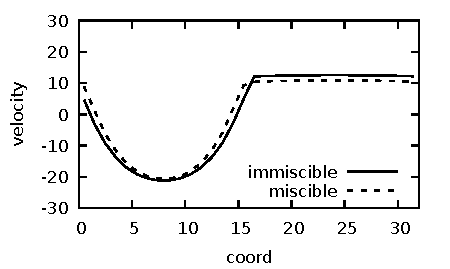
\includegraphics[width=0.6\textwidth]{i/flow/prof.pdf}
\end{center}
